\documentclass{beamer}
\usepackage[unilu,en]{collegeBeamer}
\usepackage[backend=biber]{biblatex}
\usepackage[usenames,dvipsnames]{xcolor}
\setbeamertemplate{footline}[frame number]
\usepackage{graphicx}
\usepackage{tikz}
\usetikzlibrary{calc, arrows.meta, intersections, patterns, positioning, shapes.misc, fadings, through, decorations.pathreplacing}
\usepackage{etoolbox}

\addbibresource{references.bib}

% meta-data
\title{GraphSAGE}
\subtitle{Inductive Representation Learning\\on Large Graphs}
\author{Thomas Gantz\\Alberto Finardi\\Tommaso Crippa\\Jan Marxen}
\date{\today}
\themecolor{50,50,50}

% document body
\begin{document}

\maketitle

%-----------------------------------------------------------------------
\section{Introduction}
%-----------------------------------------------------------------------

\begin{frame}{Graph Prediction Tasks}
    \begin{columns}
        \begin{column}{0.55\textwidth}
            \textbf{Primary focus:} Node-level prediction — predict properties of individual nodes (classification, regression).
            
            \vspace{10pt}
            \begin{itemize}
                \item \textbf{Node-level (focus):} Predict node attributes or labels using features and neighbor information.
                \item \textbf{Edge-level:} Predict relationships between node pairs (link prediction, edge classification).
                \item \textbf{Graph-level:} Predict properties of whole graphs (e.g., molecule properties).
            \end{itemize}
        \end{column}
        \begin{column}{0.42\textwidth}
            \centering
            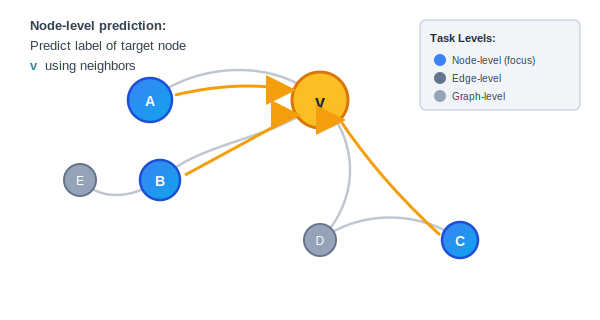
\includegraphics[width=1.2\textwidth]{img/graph_prediction_light.png}
        \end{column}
    \end{columns}
\end{frame}

\begin{frame}{What is a Graph Neural Network?}

    \vspace{4pt}
    \textbf{A learnable transformation} on graph attributes that:
    \begin{itemize}
        \item Updates node/edge/graph features using \textbf{neural networks}
        \item \textbf{Respects graph structure} by aggregating information from neighbors
        \item Is \textbf{permutation invariant} (order of nodes doesn't matter)
    \end{itemize}
    
    \vspace{5pt}
    \centering
    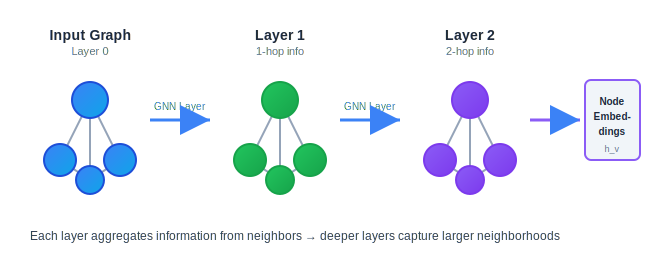
\includegraphics[width=0.75\textwidth]{img/gnn_layer_transform_light.png}
\end{frame}

\begin{frame}{Message Passing: The Core Idea}
    \textbf{Three steps repeated at each layer:}
    \begin{enumerate}
        \item \textbf{Gather:} Collect embeddings from neighboring nodes
        \item \textbf{Aggregate:} Combine neighbors' info (sum / mean / max)
        \item \textbf{Update:} Apply learned transform using the aggregated vector
    \end{enumerate}
    
    \vspace{10pt}
    \begin{block}{Message Passing Equation}
        \centering
        $h_v^{(k)} = \sigma\left( W \cdot \left[ h_v^{(k-1)} \, , \, \mathrm{AGG}\left(\{ h_u : u \in N(v) \}\right) \right] \right)$
    \end{block}
    
    \vspace{10pt}
    \small
    \textit{Analogy: CNNs aggregate over fixed local pixel neighborhoods; GNNs aggregate over variable-size neighbor sets.}
\end{frame}

\begin{frame}{Message Passing: Notation}
    \begin{columns}
        \begin{column}{0.48\textwidth}
            \begin{itemize}
                \item $h_v^{(k)}$ — Representation of node $v$ at layer $k$
                \item $h_u$ — Representation of neighbor node $u$
                \item $N(v)$ — Set of neighbor nodes of $v$
                \item $k$ — Layer index (message-passing hops)
            \end{itemize}
        \end{column}
        \begin{column}{0.48\textwidth}
            \begin{itemize}
                \item $\mathrm{AGG}(\cdot)$ — Aggregator function (mean, sum, max, LSTM)
                \item $W$ — Learnable weight matrix
                \item $\sigma$ — Non-linear activation (ReLU, tanh)
            \end{itemize}
        \end{column}
    \end{columns}
\end{frame}

\begin{frame}{Before GraphSAGE: The Problem}
    \textit{Let's audit the limitations of existing approaches...}
    
    \vspace{12pt}
    \begin{itemize}
        \item \textbf{DeepWalk / node2vec:} Transductive: embed every node; new nodes need full retraining.\\
              \hspace{1em}{\small \textcolor{gray}{$\triangleright$ Not GNNs — random-walk based embeddings, no message passing}}
        \item \textbf{GCNs:} Often require access to the full graph during training/inference; can be costly to scale.\\
              \hspace{1em}{\small \textcolor{gray}{$\triangleright$ GNNs — but transductive: fixed node set at training}}
        \item \textbf{Result:} No compact parametric function to generate embeddings for unseen nodes.
    \end{itemize}
    
    \vspace{12pt}
    \textit{This motivates GraphSAGE's key insight...}
\end{frame}

%-----------------------------------------------------------------------
\section{The Key Insight}
%-----------------------------------------------------------------------

\begin{frame}{The Key Insight}
    \centering
    \vspace{5pt}
    
    {\Large \textbf{Don't learn embeddings for each node...}}
    
    \vspace{10pt}
    
    {\Large \textcolor{orange}{\textbf{Learn a FUNCTION that generates embeddings}}}
    
    \vspace{8pt}
    
    \textit{By sampling \& aggregating neighborhood features}
    
    \vspace{8pt}
    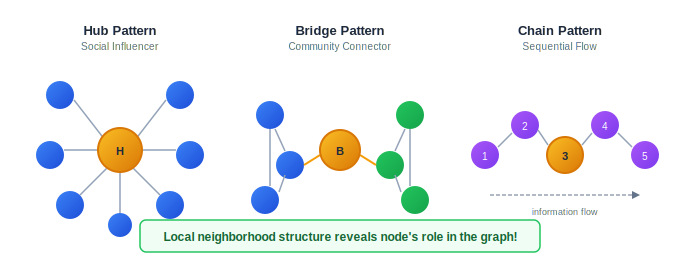
\includegraphics[width=0.65\textwidth]{img/graphs_examples_light.png}
\end{frame}

%-----------------------------------------------------------------------
\section{GraphSAGE Framework}
%-----------------------------------------------------------------------

\begin{frame}{GraphSAGE: Inductive Framework}
    \textbf{Core Principle:} Sample + Aggregate
    
    \vspace{10pt}
    \begin{itemize}
        \item Learn \textbf{aggregator functions} (not node embeddings)
        \item For any node $v$: \textbf{sample neighbors, aggregate their features}
        \item Pass through learned neural networks
        \item \textbf{Inference:} Apply same function to unseen nodes
    \end{itemize}
    
    \vspace{10pt}
    \centering
    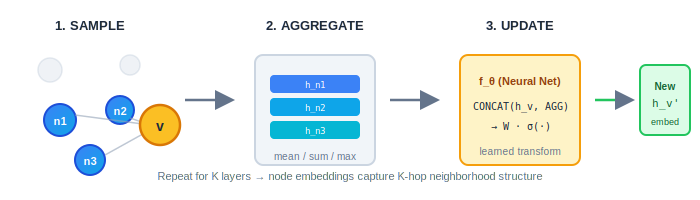
\includegraphics[width=0.95\textwidth]{img/graphsage_sample_aggregate_light.png}
\end{frame}

%-----------------------------------------------------------------------
\section{Implementation}
%-----------------------------------------------------------------------

\begin{frame}{Implementation}
    \centering
    \vspace{30pt}
    {\Large \textit{Implementation details coming soon...}}
    \vspace{30pt}
\end{frame}

%-----------------------------------------------------------------------
\section{Hyperparameters}
%-----------------------------------------------------------------------

\begin{frame}{Hyperparameters}
    \centering
    \vspace{30pt}
    {\Large \textit{Hyperparameter tuning details coming soon...}}
    \vspace{30pt}
\end{frame}

%-----------------------------------------------------------------------
\section{Results}
%-----------------------------------------------------------------------

\begin{frame}{Results}
    \centering
    \vspace{30pt}
    {\Large \textit{Experimental results coming soon...}}
    \vspace{30pt}
\end{frame}

%-----------------------------------------------------------------------
\QApage

\bibliographpage

\end{document}
